% DSD Lab3 report

\documentclass[10pt]{article}
\usepackage{mathtools, amsmath, amsfonts, amssymb}
\usepackage{hyperref, graphicx, wrapfig, geometry}
\usepackage[makeroom]{cancel}

\usepackage[section]{placeins}
\newgeometry{margin=2cm}

\title{ECSE 323 --- Group 47 Lab 4 Report Permutation}
\author{Jun Young Shin id. 260499663\\ Timothee Flichy id. 260557686}
\date{\today}

\begin{document}
\maketitle
\section{On-Chip Testing using the SignalTap II Logic Analyzer}
During our on-chip testing of the enigma, when everything was well setup, the test output of the test bed when the reset key was pressed, we where only getting one portion of the entire cycle of the counter. The TA could not explain what was going on even though the VHDL code was working perfectly on the Altera board when we uploaded the code to it.

\section{Permutation}
The permutation is used to both encode and decode the input letter. To do so, we were given a table which depicts the character encryption list given in the figure \ref{fig:permuation}. We were told to implement the first 4 rotor types. To make the permutation circuit, we need 2 input and 2 outputs. The inputs will receive a 2 bit rotor\_type and the second input is a 5-bit input\_code (letter) that must be encrypted. The outputs are a 5 bit output\_code which outputs the encrypted version of the input bits determined by the rotor position and the second input is the inv\_output\_code giving the inverted or decrypted 5 bit code. This is given by the figure \ref{fig:permuation_sym}.
\begin{figure}[!htb]
    \centering
    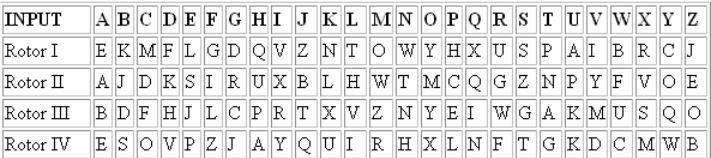
\includegraphics[width=0.5\textwidth]{./permutation.png}
    \caption{Permutation graph.}
    \label{fig:permuation}
\end{figure}
\begin{figure}[!htb]
    \centering
    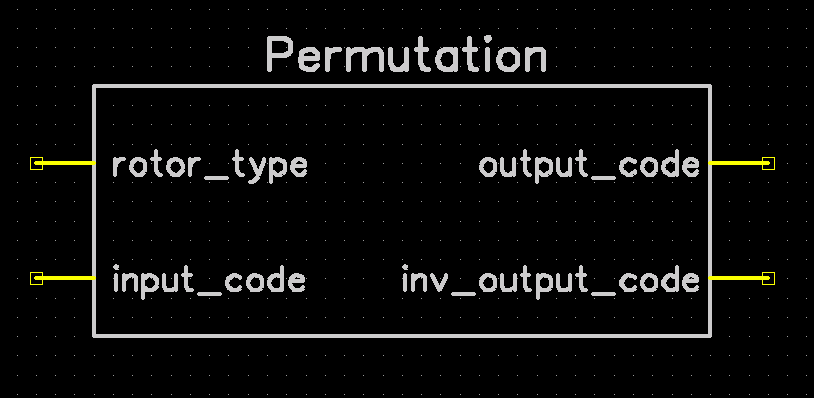
\includegraphics[width=0.5\textwidth]{./permutation_circuit.png}
    \caption{Permutation symbol.}
    \label{fig:permuation_sym}
\end{figure}
We tested out vhdl code on the ModelSim and got what we were expected to get from the permutation graph as you can see from the figures \ref{fig:perm_1}, \ref{fig:perm_2}, \ref{fig:perm_3}, \ref{fig:perm_4}, and \ref{fig:perm_5}.
\begin{figure}[!htb]
    \centering
    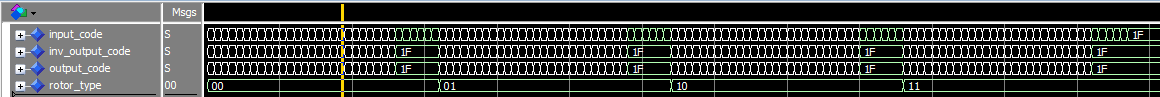
\includegraphics[width=1\textwidth]{./perm_1.png}
    \caption{Tested circuit on ModelSim}
    \label{fig:perm_1}
\end{figure}
\begin{figure}[!htb]
    \centering
    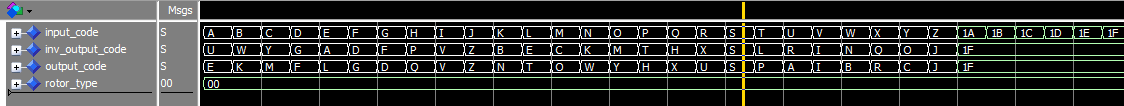
\includegraphics[width=1\textwidth]{./perm_2.png}
    \caption{With rotor I.}
    \label{fig:perm_2}
\end{figure}
\begin{figure}[!htb]
    \centering
    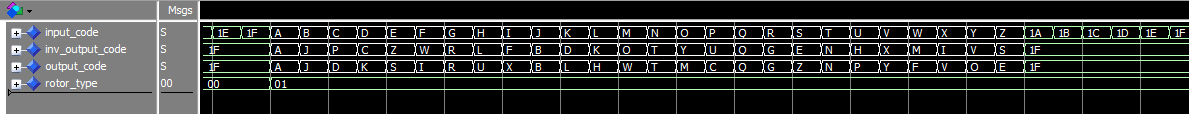
\includegraphics[width=1\textwidth]{./perm_3.png}
    \caption{With rotor II.}
    \label{fig:perm_3}
\end{figure}
\begin{figure}[!htb]
    \centering
    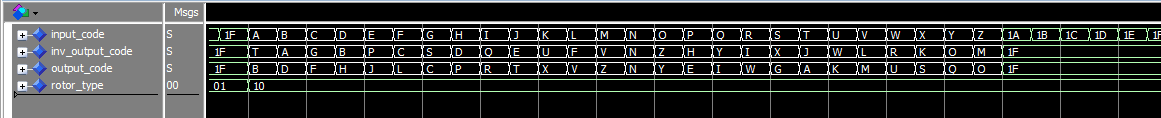
\includegraphics[width=1\textwidth]{./perm_4.png}
    \caption{With rotor III.}
    \label{fig:perm_4}
\end{figure}
\begin{figure}[!htb]
    \centering
    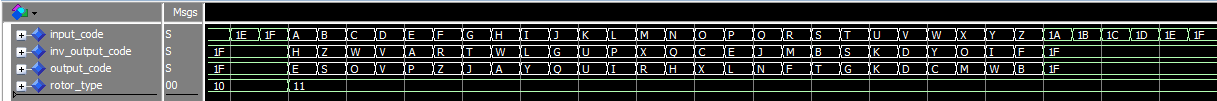
\includegraphics[width=1\textwidth]{./perm_5.png}
    \caption{With rotor IV.}
    \label{fig:perm_5}
\end{figure}

\section{fsm}
For the Finite State Machine circuit (FSM), we built a circuit that performed the requirements mentioned on the lab sheet. The states are as following shown in the figure \ref{fig:state_diagram}.
\begin{figure}[!htb]
    \centering
    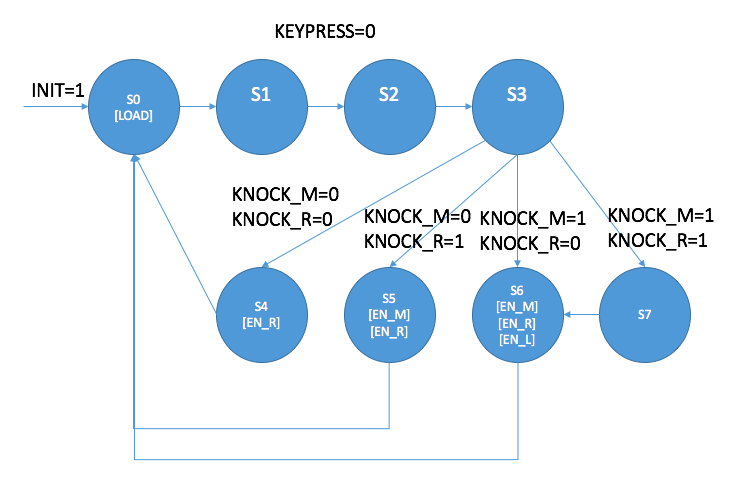
\includegraphics[width=0.5\textwidth]{./state_diagram.png}
    \caption{State Diagram.}
    \label{fig:state_diagram}
\end{figure}
To make this work, we wrote a FSM where we have 5 inputs and 4 outputs as shown in the figure \ref{fig:FSM}.
\begin{figure}[!htb]
    \centering
    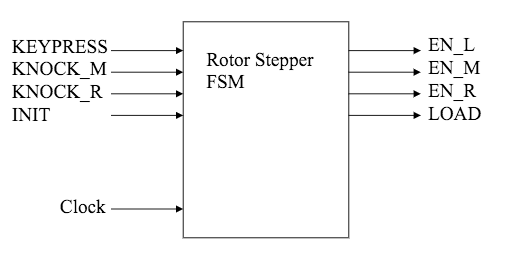
\includegraphics[width=0.5\textwidth]{./FSM.png}
    \caption{FSM symbol.}
    \label{fig:FSM}
\end{figure}
Circuit goes as follows. The circuit checks for the INIT to go high. When INIT is high, the LOAD will go high. After this, it waits for the KEYPRESS to go low (the Altera board is active high). Next it checks the KNOCK\_M and KNOCK\_R. When both KNOCK values are low, then only the EN\_R is set high. When only KNOCK\_R is high, then the EN\_R and EN\_M is set high. When only KNOCK\_M is high, the all EN is go high. When both KNOCK's are high, is will go to the state where all EN are high. After the states where EN are set, it will return to state 1 (where it waits) and start over again. At this point the INIT does not need to be checked. The figure \ref{fig:fsm_test} shows the circuit in a simulated environment.
\begin{figure}[!htb]
    \centering
    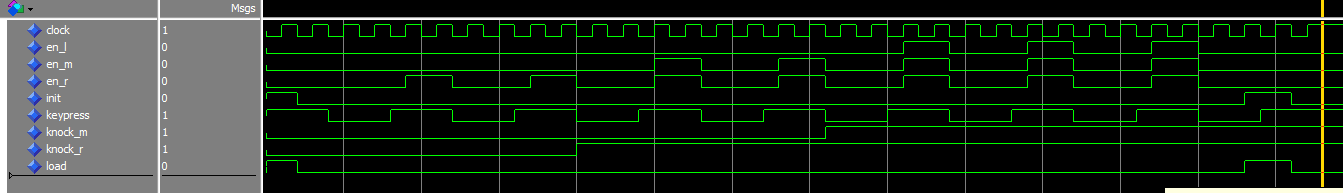
\includegraphics[width=1\textwidth]{./fsm_test.png}
    \caption{FSM symbol.}
    \label{fig:fsm_test}
\end{figure}
To the run the circuit, we have found in the slow model that Fmax=75.04MHz, Setup slack to be 3.337 ns, and hold time of 0.445 ns. In the fast model, setup time is 7.848 ns and hold time to be 0.215 ns.


\end{document}
